\chapter{Fundamentação Teórica}\label{fundamentacaoTeorica}

Neste capítulo é apresentado de forma abrangente os domínios abordados para a realização e compreensão deste trabalho. 
A Seção \ref{sec:ProjetoBD} expõe o que é um projeto de \acp{BD} e suas fases de modelagem para a construção de esquemas de \acp{BD}. 
A Seção \ref{sec:LinguagemSQL} elucida a aplicação da \ac{SQL}, e exemplifica seu uso com alguns exemplos de \acp{SGBD}. 
A Seção \ref{ssec:MDE} aborda a Engenharia Dirigida por Modelos, do inglês \ac{MDE}, e suas aplicações com as \acp{DSL}. 
Na Seção \ref{sec:TrabRelacionados} é discutido os trabalhos relacionados e, por fim, na Seção \ref{sec:LicoesFundamentacaoTeorica} é apresentado algumas lições aprendidas e pontuados os principais tópicos discutidos.

%#################################################################
\section{Projeto de Banco de Dados} \label{sec:ProjetoBD}
%#################################################################

Segundo \citeonline{Date:2004} um \ac{BD} é fundamentalmente um sistema computacional para a manutenção de registros. 
Sistemas desse tipo tem a finalidade de armazenar dados de forma persistente, bem como permitir que usuários definam, busquem e atualizem esses dados para gerar informações pertinentes quando necessário. 
Um \ac{BD} pode ser representado por um modelo de dados, expressado em diferentes níveis e com diferentes técnicas.

Normalmente durante o ciclo de desenvolvimento de software os modelos de dados passam por níveis distintos de transformações. 
Inicialmente não existia um padrão ou recomendação difundida amplamente na indústria, ou mesmo na academia, para o processo de modelagem de dados. 
A estratégia para a utilização de diferentes níveis de projeto e representação tem suas origens com o grupo de estudos em \acp{SGBD} intitulado \textit{ANSI/X3/SPARK}, ainda na década de 1970 \cite{DBLP:1975}.  

Na abordagem proposta, o padrão de definição e especificação de parâmetros e elementos que compreendiam um \ac{BD} levavam em consideração aspectos conceituais, lógicos e físicos. 
Esses aspectos eram chamados genericamente de esquemas (do inglês, \textit{schemas}). 
Esses esquemas na realidade eram fragmentos que serviam, quando em conjunto, para todo o mapeamento da estrutura de um \ac{BD}. 
Esses mesmos conceitos continuam em aplicação até os dias de hoje na implementação de \acp{BD} em \acp{SGBD}.  

De acordo com \citeonline{Cougo:2013}, as dificuldades existentes antes do estabelecimento da arquitetura de três níveis estava essencialmente em um ponto. 
Um mesmo modelo de dados concebido para uma aplicação necessitava de diferentes implementações quando aplicados aos \acp{SGBD} primitivos da época anterior a proposta de três níveis, incluindo modificações significativas no próprio modelo original. 
Isso ocasionava como resultado esquemas bastante particulares e reflexos significativos no modelo de dados final.

Tendo essa realidade como fato, um mesmo modelo de dados gerado para uma única aplicação poderia necessitar de um grande número de diferentes esquemas para abranger as variações de modos de implementação e de visões externas a serem disponibilizadas aos usuários. 
As dificuldades provenientes da administração e manutenção de toda essa variedade de modelos levaram o grupo \textit{ANSI/X3/SPARK} a propor o padrão que tem como ideia central a definição de níveis de esquemas relacionados a um modelo de dados \cite{Cougo:2013}.
Esse padrão acabou por influenciar a proposta de modelagem conceitual de dados concebida por \citeonline{Chen:1976}. 
Sendo assim, os \acp{BD} relacionais até os dias atuais continuam levando em consideração estes conceitos. 

A construção de um \ac{BD} é baseada em um modelo de \ac{BD}, o qual é uma descrição detalhada dos tipos de informações que devem ser armazenadas. 
O projeto de \ac{BD} acontece em três fases distintas de modelagem, onde são gerados o \ac{MCD}, \ac{MLD} e o \ac{MFD} \cite{Heuser:2009}. 
Para a elaboração de modelos de dados deve ser usado uma linguagem de modelagem de dados. 
Existem linguagens gráficas e textuais capazes de descrever os modelos em diferentes níveis de detalhamento e abstração.  

%Entre as vantagens da abordagem de \acp{BD}, \citeonline{Date:2004} enumera as seguintes: (I)Os dados podem ser compartilhados; (II)A redundância de dados pode ser reduzida; (III)A inconsistência pode ser evitada, pelo menos até certo ponto; (IV)O suporte a transações pode ser fornecido; (V)A integridade pode ser mantida; (VI)A segurança pode ser reforçada; (VII)Requisitos podem ser equilibrados; e (VIII)Os padrões podem ser impostos.  

%#################################################################
\subsection{Modelo Conceitual de Dados} \label{ssec:ModelConceitual}
%#################################################################

O \ac{MCD} é a descrição do \ac{BD} de forma independente da implementação utilizada em um \ac{SGBD}. 
Este modelo lista quais dados podem ocorrer no \ac{BD}, mas não registra como estes dados estão armazenados no nível de \ac{SGBD}. 
A técnica mais difundida de \ac{MCD} é a \ac{ER} de \citeonline{Chen:1976}. 
Esta abordagem foi tão bem aceita que passou a ser considerada uma referência definitiva para a modelagem de \acp{BD} relacionais. 
É composta basicamente por um método de diagramação e de conceitos que devem ser respeitados. 
Sendo assim, com esta abordagem os \acp{MCD} são representados com \acp{DER}, como pode ser visto na \autoref{fig:DER}.
    
\begin{figure}[htb]
	\centering
	\caption{Fragmento de DER.}
		\includegraphics[width=0.6\textwidth]{img/MCD.jpg}
	\fonte{\citeonline{Heuser:2009}.}
	\label{fig:DER}
\end{figure}

Na abordagem \ac{ER} o conceito principal é o de \textbf{entidade}, o qual é uma representação de um conjunto de objetos do domínio modelado. 
As entidades são simbolizadas por retângulos. 
Contudo, nesta abordagem ainda existem também outros conceitos que são essenciais e devem ser analisados.

Os \textbf{relacionamentos} representam a associação entre os objetos e são sinalizados por losangos. 
A \textbf{cardinalidade} de relacionamentos registra o número de ocorrências com que as entidades podem se associar. 
Existem duas cardinalidades que devem ser atribuídas: a mínima e a máxima. Os \textbf{atributos} são características representadas por pequenos círculos conectados as entidades. 
Na esquerda da \autoref{fig:DER2} é ilustrado um exemplo de \ac{DER} simples e, na direita, uma representação hipotética do conjunto de ocorrências que podem acontecer entre suas entidades. 

\begin{figure}[htb]
	\centering
	\caption{Relacionamentos e cardinalidades.}
		\includegraphics[width=0.5\textwidth]{img/RelCard.jpg}
	\fonte{\citeonline{Heuser:2009}.}
	\label{fig:DER2}
\end{figure}

%#################################################################
    \subsection{Modelo Lógico de Dados} \label{ssec:ModelLogico}
%#################################################################

Um \ac{MLD} é definido como um modelo que possui a representação dos objetos, relacionamentos e características de acordo com regras de implementação. 
Isso significa que esse modelo tem um nível de abstração do ponto de vista do usuário de um \ac{SGBD}. 
Ainda assim, o modelo lógico é independente do tipo de \ac{SGBD} em que é implementado. 
Na \autoref{fig:MLD} é apresentado um \ac{MLD} gráfico baseado no modelo da \autoref{fig:DER}.

\begin{figure}[htb]
	\centering
	\caption{Exemplo de MLD.}
		\includegraphics[width=0.8\textwidth]{img/MLD.jpg}
	\fonte{\citeonline{Heuser:2009}.}
	\label{fig:MLD}
\end{figure}

Esse tipo de modelo deve necessariamente respeitar conceitos tais como chaves de acesso, controle de chaves duplicadas, normalização, integridade referencial, controle de redundância de dados, entre outros. 
Este modelo é intrinsecamente relacionado a fase de projeto \cite{Cougo:2013}. 
É importante salientar que essa é uma forma direcionada a um aspecto gráfico, porém existem meios alternativos de se representar estruturalmente o mesmo modelo de forma textual \cite{Martelli:2018}. 
Isso é mostrado na \autoref{fig:LogicoTextual} que apresenta a definição da mesma estrutura descrita na \autoref{fig:MLD}.

\begin{figure}[!htb]
    \caption{Estrutura de um modelo lógico descrita de forma textual.}
    \label{fig:LogicoTextual}
    \centering
    \fbox{
        \parbox{13cm}{
        TipoDeProduto (\underline{CodTipoProd}, DescrTipoProd)\\
        Produto (\underline{CodProd}, DescrProd, PrecoProd, CodTipoProd)\\
        CodTipoProd referencia TipoDeProduto
        }}    
    \fonte{\citeonline{Heuser:2009}.}
\end{figure}

A obtenção de um \ac{MLD} se dá mediante a aplicação de regras de derivação sobre um \ac{MCD} já construído. 
Entretanto, não é raro que desenvolvedores e analistas experientes comecem diretamente pelo processo de modelagem lógica, ignorando a modelagem conceitual. 
Isso ocorre pois esse modelo não se preocupa somente com a representação dos objetos observados no domínio analisado, mas também com outros elementos como chaves, métodos de acesso, formatos de campo, etc. 
Isso implica, em uma última observação, que do ponto de vista formal da definição da abordagem \ac{ER}, esse modelo não se enquadra fielmente como um modelo \ac{ER} \cite{West:2011}.

%#################################################################
    \subsection{Modelo Físico de Dados} \label{ssec:ModelFisico}
%#################################################################

Um \ac{MFD} caracteriza-se como um modelo em que a representação dos objetos de \ac{BD} já estão em um nível físico de implementação das ocorrências, ou instâncias, das entidades de relacionamentos. 
Cada \ac{SGBD} pode definir diferentes modos de implementação física das características e recursos indispensáveis para o armazenamento e manipulação das estruturas de dados \cite{Cougo:2013}.

Em geral os modelos físicos apresentam dois aspectos bem representados. 
Primeiramente, existem as ocorrências ou instâncias, seus relacionamentos e a disposição básica dos elementos. 
O outro aspecto diz respeito a alocação nos diversos níveis de agrupamentos possíveis, como as tabelas, linhas (registros), colunas (campos) e blocos \cite{West:2011}.
Em suma é uma sequência lógica de instruções em \ac{SQL}, executadas em um \ac{SGBD}.

%#################################################################
\section{Linguagem SQL} \label{sec:LinguagemSQL}
%#################################################################

Para a manipulação dos dados a \ac{SQL} é a linguagem padrão utilizada por sistemas de \acp{BD} relacionais disponíveis no mercado. 
A \ac{SQL} teve sua gênese originalmente nos laboratórios da IBM Research, na década de 1970, com o nome inicial de SEQUEL \cite{Chamberlin:1974}.
A \ac{SQL} é uma linguagem com a versão estável mais recente lançada em 2016 e denominada \texttt{SQL:2016}, possuindo um total de mais de 2000 páginas de especificação\footnote{https://iso.org/standard/63555.html}\footnote{https://standards.iso.org/ittf/PubliclyAvailableStandards/c065143_ISO_IEC_TR_19075-5_2016.zip}\footnote{https://standards.iso.org/ittf/PubliclyAvailableStandards/c067367_ISO_IEC_TR_19075-6_2017.zip}\footnote{https://standards.iso.org/ittf/PubliclyAvailableStandards/c069776_ISO_IEC_TR_19075-7_2017.zip}. 
Entretanto, é importante salientar que ao mesmo tempo em que a maioria dos produtos do mercado trabalham com a \ac{SQL}, estas soluções também deixam de oferecer suporte a determinados aspectos ou ainda os implementa de uma forma diferente da especificação oficial. 

A \ac{SQL} é uma única linguagem, mas comumente é categorizada conforme a funcionalidade das suas instruções. 
A primeira categoria é chamada Linguagem de Definição de Dados, do inglês \ac{DDL}. 
Entre os comandos dessa categoria estão o \texttt{CREATE}, \texttt{ALTER}, \texttt{DROP} e \texttt{TRUNCATE}. 
A segunda categoria é nomeada de Linguagem de Definição de Dados, do inglês \ac{DML}. 
Entre os comandos categorizados como \ac{DML} estão o \texttt{INSERT}, \texttt{UPDATE} e \texttt{DELETE}. 
A terceira categoria é chamada de Linguagem de Consulta de Dados, do inglês \ac{DQL}, a qual possui apenas o comando \texttt{SELECT}. 
A quarta categoria é denominada Linguagem de Transação de Dados, do inglês \ac{DTL}, a qual detém comandos como \texttt{COMMIT} e \texttt{ROLLBACK}.

A \ac{SQL} ainda utiliza uma série de cláusulas (\textit{e.g.} \texttt{FROM}, \texttt{WHERE}, \texttt{GROUP BY}, \texttt{ORDER BY}, \texttt{HAVING}, \texttt{DISTINCT}, \texttt{UNION}), operadores lógicos (\textit{e.g.} \texttt{AND}, \texttt{OR}, \texttt{NOT}), operadores relacionais (\textit{e.g.} \texttt{<}, \texttt{>}, \texttt{<=}, \texttt{>=}, \texttt{=}, \texttt{<>}) e funções de agregação (\textit{e.g.} \texttt{AVG}, \texttt{SUM}, \texttt{COUNT}, \texttt{MAX}, \texttt{MIN}). 
A aplicação destes termos e palavras reservadas, associado a características inspiradas na álgebra relacional, fundamenta a base da \ac{SQL} utilizada pelos \acp{SGBD}.

%#################################################################
    \subsection{Bancos de Dados Relacionais} \label{ssec:SGBDRelacionais}
%#################################################################

Os \acp{SGBD} relacionais suportam o modelo de dados relacional. 
O modelo de dados relacional foi proposto por \citeonline{Codd:1970} e tem como premissa a modelagem orientada a tabelas. 
Um ponto importante a ser citado é o fato de praticamente todos os \acp{SGBD} relacionais do mercado utilizarem \ac{SQL} para a criação e manipulação dos dados.

\begin{figure} [!htb]
    \centering
    \caption{Modelo de dados relacional.}
    \label{fig:ModeloRelacional}
    

\tikzset{every picture/.style={line width=0.75pt}} %set default line width to 0.75pt        

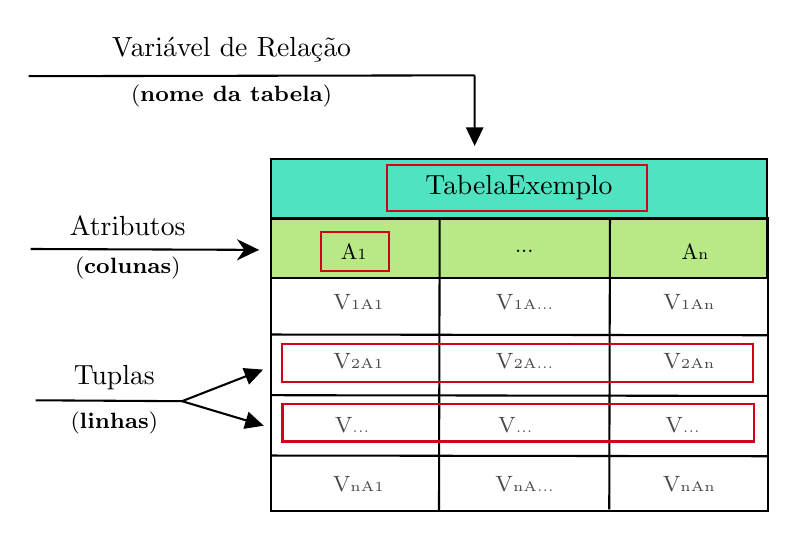
\begin{tikzpicture}[x=0.75pt,y=0.75pt,yscale=-1,xscale=1]
%uncomment if require: \path (0,456.4000015258789); %set diagram left start at 0, and has height of 456.4000015258789

%Shape: Rectangle [id:dp9895438777319416] 
\draw   (199.76,128.06) -- (439.3,128.06) -- (439.3,269.14) -- (199.76,269.14) -- cycle ;
%Straight Lines [id:da9433008870660626] 
\draw    (200.17,183.96) -- (439.3,184.31) ;


%Straight Lines [id:da2966959811071168] 
\draw    (199.96,213.19) -- (439.09,213.54) ;


%Straight Lines [id:da10336227761172356] 
\draw    (199.96,242.26) -- (439.09,242.6) ;


%Shape: Rectangle [id:dp29843450985148356] 
\draw  [fill={rgb, 255:red, 184; green, 233; blue, 134 }  ,fill opacity=1 ] (199.76,128.06) -- (439.07,128.06) -- (439.07,156.8) -- (199.76,156.8) -- cycle ;
%Straight Lines [id:da7072311505307143] 
\draw    (281.21,128) -- (280.87,268.53) ;


%Straight Lines [id:da24303755507006675] 
\draw    (363.25,127.67) -- (362.9,268.19) ;


%Straight Lines [id:da8433947995405431] 
\draw    (84.07,142.75) -- (192.19,143.17) ;
\draw [shift={(194.19,143.18)}, rotate = 180.22] [fill={rgb, 255:red, 0; green, 0; blue, 0 }  ][line width=0.75]  [draw opacity=0] (10.72,-5.15) -- (0,0) -- (10.72,5.15) -- (7.12,0) -- cycle    ;

%Shape: Rectangle [id:dp9829425897866726] 
\draw  [color={rgb, 255:red, 208; green, 2; blue, 27 }  ,draw opacity=1 ] (205.49,217.22) -- (432.44,217.22) -- (432.44,235.51) -- (205.49,235.51) -- cycle ;
%Straight Lines [id:da9003126370670107] 
\draw    (86.49,215.65) -- (157.07,216.08) ;


%Shape: Rectangle [id:dp34368494625131474] 
\draw  [color={rgb, 255:red, 208; green, 2; blue, 27 }  ,draw opacity=1 ] (205.06,188.46) -- (432,188.46) -- (432,206.75) -- (205.06,206.75) -- cycle ;
%Straight Lines [id:da28450929807989755] 
\draw    (157.07,216.08) -- (194.24,201.59) ;
\draw [shift={(196.1,200.87)}, rotate = 518.71] [fill={rgb, 255:red, 0; green, 0; blue, 0 }  ][line width=0.75]  [draw opacity=0] (8.93,-4.29) -- (0,0) -- (8.93,4.29) -- cycle    ;

%Straight Lines [id:da38844388554414944] 
\draw    (157.07,216.08) -- (194.52,227.29) ;
\draw [shift={(196.43,227.87)}, rotate = 196.67000000000002] [fill={rgb, 255:red, 0; green, 0; blue, 0 }  ][line width=0.75]  [draw opacity=0] (8.93,-4.29) -- (0,0) -- (8.93,4.29) -- cycle    ;

%Straight Lines [id:da6694551113867799] 
\draw    (83.2,59.49) -- (298.05,59.09) ;


%Shape: Rectangle [id:dp5574880153243091] 
\draw  [fill={rgb, 255:red, 80; green, 227; blue, 194 }  ,fill opacity=1 ] (199.76,99.32) -- (439.07,99.32) -- (439.07,128.06) -- (199.76,128.06) -- cycle ;
%Straight Lines [id:da8765291155015824] 
\draw    (298.05,59.09) -- (298.06,91.08) ;
\draw [shift={(298.06,93.08)}, rotate = 269.98] [fill={rgb, 255:red, 0; green, 0; blue, 0 }  ][line width=0.75]  [draw opacity=0] (8.93,-4.29) -- (0,0) -- (8.93,4.29) -- cycle    ;

%Shape: Rectangle [id:dp31459180611157866] 
\draw  [color={rgb, 255:red, 208; green, 2; blue, 27 }  ,draw opacity=1 ] (255.94,102.46) -- (381.06,102.46) -- (381.06,124.63) -- (255.94,124.63) -- cycle ;
%Shape: Rectangle [id:dp48382611043878065] 
\draw  [color={rgb, 255:red, 208; green, 2; blue, 27 }  ,draw opacity=1 ] (224.14,134.4) -- (256.9,134.4) -- (256.9,153.28) -- (224.14,153.28) -- cycle ;

% Text Node
\draw (239.74,144.01) node [scale=0.8] [align=left] {A{\scriptsize 1}};
% Text Node
\draw (321.96,144.01) node [scale=0.8] [align=left] {...};
% Text Node
\draw (404.18,144.01) node [scale=0.8] [align=left] {A{\scriptsize n}};
% Text Node
\draw (241.98,168.48) node [scale=1,color={rgb, 255:red, 74; green, 74; blue, 74 }  ,opacity=1 ] [align=left] {{\footnotesize V}{\tiny 1A1}};
% Text Node
\draw (130.91,131.43) node [scale=1] [align=left] {Atributos};
% Text Node
\draw (130.91,151.67) node [scale=1] [align=left] {{\footnotesize (\textbf{colunas})}};
% Text Node
\draw (241.98,196.46) node [scale=1,color={rgb, 255:red, 74; green, 74; blue, 74 }  ,opacity=1 ] [align=left] {{\footnotesize V}{\tiny 2A1}};
% Text Node
\draw (238.98,227.67) node [scale=1,color={rgb, 255:red, 74; green, 74; blue, 74 }  ,opacity=1 ] [align=left] {{\footnotesize V}{\tiny ...}};
% Text Node
\draw (241.98,256.17) node [scale=1,color={rgb, 255:red, 74; green, 74; blue, 74 }  ,opacity=1 ] [align=left] {{\footnotesize V}{\tiny nA1}};
% Text Node
\draw (322.14,168.48) node [scale=1,color={rgb, 255:red, 74; green, 74; blue, 74 }  ,opacity=1 ] [align=left] {{\footnotesize V}{\tiny 1A...}};
% Text Node
\draw (322.14,196.46) node [scale=1,color={rgb, 255:red, 74; green, 74; blue, 74 }  ,opacity=1 ] [align=left] {{\footnotesize V}{\tiny 2A...}};
% Text Node
\draw (317.64,227.67) node [scale=1,color={rgb, 255:red, 74; green, 74; blue, 74 }  ,opacity=1 ] [align=left] {{\footnotesize V}{\tiny ...}};
% Text Node
\draw (322.14,256.17) node [scale=1,color={rgb, 255:red, 74; green, 74; blue, 74 }  ,opacity=1 ] [align=left] {{\footnotesize V}{\tiny nA...}};
% Text Node
\draw (401.22,168.48) node [scale=1,color={rgb, 255:red, 74; green, 74; blue, 74 }  ,opacity=1 ] [align=left] {{\footnotesize V}{\tiny 1An}};
% Text Node
\draw (401.22,196.46) node [scale=1,color={rgb, 255:red, 74; green, 74; blue, 74 }  ,opacity=1 ] [align=left] {{\footnotesize V}{\tiny 2An}};
% Text Node
\draw (398.22,227.67) node [scale=1,color={rgb, 255:red, 74; green, 74; blue, 74 }  ,opacity=1 ] [align=left] {{\footnotesize V}{\tiny ...}};
% Text Node
\draw (401.22,256.17) node [scale=1,color={rgb, 255:red, 74; green, 74; blue, 74 }  ,opacity=1 ] [align=left] {{\footnotesize V}{\tiny nAn}};
% Text Node
\draw (124.43,204.59) node [scale=1] [align=left] {Tuplas};
% Text Node
\draw (124.43,226.56) node [scale=1] [align=left] {{\footnotesize (\textbf{linhas})}};
% Text Node
\draw (180.93,46.33) node [scale=1] [align=left] {Variável de Relação};
% Text Node
\draw (180.93,69.05) node [scale=1] [align=left] {{\footnotesize (\textbf{nome da tabela})}};
% Text Node
\draw (319.41,113.34) node [scale=1] [align=left] {TabelaExemplo};


\end{tikzpicture}

    \fonte{O autor.}
\end{figure}

A \autoref{fig:ModeloRelacional} mostra o esquema estrutural de um modelo relacional. Nele uma tabela, também chamada de entidade, é definida por um nome e um número fixo de atributos com seus tipos de dados indicados. 
Cada tabela deve ter um ou mais atributos identificadores, chamado de chaves, o qual visa auxiliar na integridade referencial dos dados. 
Um registro, também chamado de ocorrência ou tupla, corresponde a uma linha na tabela e consiste nos valores de cada atributo. 
Uma relação, portanto, consiste em um conjunto de registros associados entre tabelas~\cite{Ramakrishnan:2002}.

\subsubsection{MySQL}
O MySQL é um \ac{SGBD} relacional que foi criado por uma empresa sueca chamada MySQL AB, e atualmente é desenvolvido e mantido pela Oracle. 
O desenvolvimento original do MySQL começou em 1994, mas a primeira versão do MySQL foi lançada apenas em maio de 1995. 
Foi inicialmente criada para uso pessoal do \ac{SGBD} mSQL baseado na linguagem de baixo nível. 
O MySQL é usado por muitos aplicativos da \textit{Web} orientados a \ac{BD} como o Drupal, o Joomla, o phpBB e o WordPress.
    
Entre suas funcionalidades mais relevantes estão o suporte multiplataforma, suporte SSL, \textit{stored procedures}, \textit{triggers}, \textit{views} atualizáveis, \textit{subselects}, entre outras. 
Atualmente, o MySQL está na versão 8.0, funciona sobre plataformas Windows, Linux, Solaris, macOS e FreeBSD. 
Existe a versão paga \textit{Enterprise Server} e a versão de código aberto MySQL \textit{Community Server}, gratuita e com licença GPL. 
É considerado o 2º \ac{SGBD} mais popular~\footnote{https://db-engines.com/en/system/MySQL} entre as opções do mercado pelo portal DB-Engines. 
Segundo a avaliação publicada em 2019 pela empresa de consultoria Gartner \textit{Group}\footnote{https://gartner.com/reviews/market/operational-dbms}, o MySQL possui uma avaliação de 4,5 de 5 pelo mercado.

\subsubsection{Microsoft SQL Server}
O Microsoft SQL Server é um \ac{SGBD} relacional desenvolvido e mantido pela Microsoft. 
Teve uma versão de teste foi criada em parceria com a Sybase em 1988, mas sua primeira versão para uso comercial foi lançada em abril de 1989. 
Desde de seu lançamento este \ac{SGBD} sofreu inúmeras melhorias. 
Atualmente possui diversas versões disponibilizadas no mercado, como a \textit{Enterprise}, a \textit{Standard}, \textit{Web}, \textit{Business Intelligence} e \textit{Workgroup}. 
    
Também possui uma versão chamada \textit{Express}, uma edição gratuita e reduzida. 
Essa versão inclui o mecanismo de \ac{BD} principal e, embora não haja limitações quanto ao número de \acp{BD} ou usuários com suporte, ele é limitado ao uso de um processador, 1 GB de memória e 10 GB de arquivos de \ac{BD}. 
O Microsoft SQL Server pode funcionar sobre plataformas Linux, Microsoft Windows Server e Microsoft Windows.
Atualmente está na versão SQL Server 2017 e é considerado o 3º \ac{SGBD} mais popular~\footnote{https://db-engines.com/en/system/Microsoft+SQL+Server} no mercado pelo portal DB-Engines. 
Segundo a avaliação publicada pela Gartner Group, o Microsoft SQL Server possui uma avaliação de 4,4 de 5 pelo mercado em 2019.

\subsubsection{PostgreSQL}
O PostgreSQL é um \ac{SGBD} que incorpora o modelo relacional para seus esquemas de dados e suporta a linguagem de consulta padrão \ac{SQL}. 
Surgiu dentro do projeto do Ingres, outro \ac{SGBD}, na universidade da Califórnia. 
Lançado em 1996 e mantido atualmente pelo PostgreSQL Global Development Group, é considerado pelo mercado um \ac{SGBD} estável, abrangente e possuidor de boas características de desempenho. 
É executado em praticamente qualquer plataforma Linux, macOS e Microsoft Windows. 
O grande diferencial do PostgreSQL para ser um dos \acp{SGBD} de maior sucesso é o fato de ser gratuito e de código aberto por meio da flexível licença BSD.
    
Entre algumas características suportadas pelo PostgreSQL estão transações, \textit{subselects}, \textit{views}, integridade referencial de chaves estrangeiras, bloqueios sofisticados, tipos definidos pelo usuário, herança, regras variadas, \textit{triggers}, funções, procedimentos armazenáveis, entre outras. 
Atualmente está na versão 11.3 e é considerado o 4º mais popular~\footnote{https://db-engines.com/en/system/PostgreSQL} entre os \acp{SGBD} existentes pelo portal DB-Engines. 
Segundo a avaliação publicada pela Gartner Group, o Microsoft SQL Server possui uma avaliação de 4,5 de 5 pelo mercado em 2019.

%#################################################################
\section{\textit{Model-Driven Engineering}} \label{ssec:MDE}
%#################################################################

Conceitualmente um modelo é uma representação, protótipo ou exemplo que se tem por objetivo reproduzir ou imitar de alguma forma. 
A construção de modelos são pontos centrais e importantes em diferentes áreas científicas. 
Na matemática, física e química, por exemplo, o emprego de modelos é tido como vital para a investigação teórica e prática em diferentes campos de estudo \cite{Bailer:2009}.

Em uma análise mais profunda, \citeonline{Brambilla:2017} discutem que, considerando-se a premissa de que um observador e suas observações alteram a própria realidade, é possível se concluir que tudo na percepção de um indivíduo é um modelo, já que absolutamente nada pode ser processado pela mente humana sem ser modelado. 
Em resumo, a criação de modelos é uma tarefa de abstração de domínios e conceitos do mundo real. %\cite{MS:2013}. 
Sendo assim, não é de surpreender que os modelos tenham se tornado cruciais e amplamente adotados também em áreas técnicas como mecânica, engenharia civil e, por fim, na ciência da computação, engenharia da computação e \ac{ES}.

A \ac{MDE}, também chamada de \ac{MDSE}, é uma abordagem da \ac{ES} para desenvolvimento de \textit{software} que tem essencialmente modelos como saídas principais de algum processo. 
Essa abordagem resulta em programas ou atividades de computador executados em \textit{hardware} ou \textit{software} que são gerados automaticamente a partir de modelos \cite{Sommerville:2011}. 
Conceitualmente, a \ac{MDE} fornece apoio a outros conceitos, como a \ac{MDD} e a \ac{MDA}. Na \autoref{fig:MDE_MDD_MDA} a relação entre estes conceitos é ilustrada.

\begin{figure}[!htb]
    \centering
    \caption{Relação de MDE, MDD e MDA.}
    \label{fig:MDE_MDD_MDA}
    

\tikzset{every picture/.style={line width=0.75pt}} %set default line width to 0.75pt        

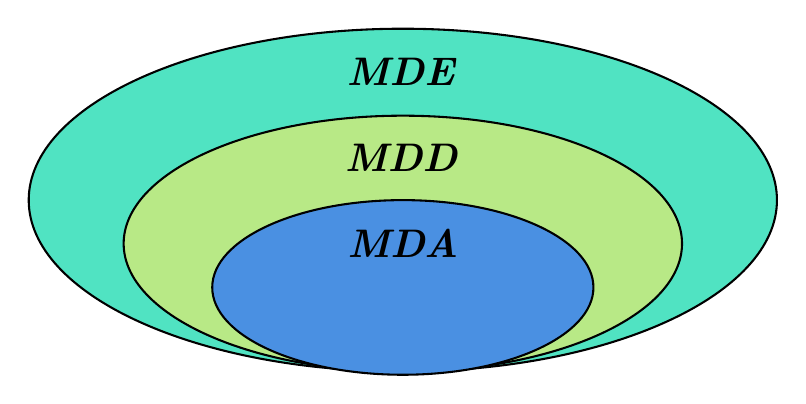
\begin{tikzpicture}[x=0.75pt,y=0.75pt,yscale=-1,xscale=1]
%uncomment if require: \path (0,300); %set diagram left start at 0, and has height of 300

%Shape: Ellipse [id:dp03875628946363818] 
\draw  [fill={rgb, 255:red, 80; green, 227; blue, 194 }  ,fill opacity=1 ] (91,113.58) .. controls (91,67.97) and (171.7,31) .. (271.25,31) .. controls (370.8,31) and (451.5,67.97) .. (451.5,113.58) .. controls (451.5,159.18) and (370.8,196.15) .. (271.25,196.15) .. controls (171.7,196.15) and (91,159.18) .. (91,113.58) -- cycle ;
%Shape: Ellipse [id:dp565416950765411] 
\draw  [fill={rgb, 255:red, 184; green, 233; blue, 134 }  ,fill opacity=1 ] (136.74,134.53) .. controls (136.74,100.49) and (196.96,72.9) .. (271.25,72.9) .. controls (345.54,72.9) and (405.76,100.49) .. (405.76,134.53) .. controls (405.76,168.56) and (345.54,196.15) .. (271.25,196.15) .. controls (196.96,196.15) and (136.74,168.56) .. (136.74,134.53) -- cycle ;
%Shape: Ellipse [id:dp0635650382067301] 
\draw  [fill={rgb, 255:red, 74; green, 144; blue, 226 }  ,fill opacity=1 ] (179.42,155.65) .. controls (179.42,132.41) and (220.53,113.58) .. (271.25,113.58) .. controls (321.97,113.58) and (363.08,132.41) .. (363.08,155.65) .. controls (363.08,178.88) and (321.97,197.72) .. (271.25,197.72) .. controls (220.53,197.72) and (179.42,178.88) .. (179.42,155.65) -- cycle ;

% Text Node
\draw (271.25,52) node [scale=1.44] [align=left] {\textit{\textbf{MDE}}};
% Text Node
\draw (271.25,93) node [scale=1.44] [align=left] {\textit{\textbf{MDD}}};
% Text Node
\draw (271.25,134.65) node [scale=1.44] [align=left] {\textit{\textbf{MDA}}};


\end{tikzpicture}

    \fonte{Adaptado de \citeonline{Ameller:2009}.}
\end{figure}

O \ac{MDD} é um paradigma de desenvolvimento que usa modelos como o principal artefato do processo de desenvolvimento. 
Normalmente na \ac{MDD} a implementação é gerada de forma semiautomática a partir dos modelos. 
Apesar de serem vistas como a mesma coisa, o conceito da \ac{MDE} tem origem na \ac{MDA}, proposta em 2001 pelo \ac{OMG}. 
Com diferenças sutis, \citeonline{Sommerville:2011} afirma que a \ac{MDA} concentra-se nos estágios de projeto e implementação do processo de desenvolvimento de software, sendo muito similar ao \ac{MDD}, porém implementando diretrizes específicas da \ac{OMG}. 
Desta forma, conclui-se que a \ac{MDA} é um subconjunto da \ac{MDD}. 
Por outro lado, a \ac{MDE} pode abordar muitos outros tópicos do processo de \ac{ES}, entre eles a engenharia de requisitos baseada em modelos, processos de software para desenvolvimento baseado em modelos, ou ainda, testes baseados em modelos.

A \ac{MDE}, como uma metodologia, auxilia a aplicação das vantagens da modelagem nas atividades de \ac{ES}. 
Para \cite{Brambilla:2017} essa abordagem leva em consideração quatro aspectos fundamentais, listados a seguir.

\begin{enumerate}
  \item \textbf{Conceitos:} os componentes que constroem a metodologia, abrangendo desde artefatos de linguagem até atores, e assim por diante;
  \item \textbf{Notações:} A maneira como os conceitos são representados, ou seja, as linguagens usadas na metodologia;
  \item \textbf{Processos e Regras:} As atividades que levam à elaboração do produto final, as regras para sua administração e controle, e as afirmações sobre as propriedades desejadas (correção, consistência, etc) dos produtos ou do próprio processo;
  \item \textbf{Ferramentas:} Aplicações que facilitam a execução de atividades ou seu controle, abrangendo o processo de produção e apoiando o desenvolvedor no uso das notações.
\end{enumerate}

A motivação por trás da \ac{MDE} é a ideia de se aumentar o nível de abstração do processo de desenvolvimento em geral, para então assim capturar sistemas ou processos como uma coleção de modelos reutilizáveis. 
Logo, ela visa reduzir a dificuldade associada ao desenvolvimento de sistemas de software, em geral mais complexos, por meio do uso de técnicas de modelagem que suportam a separação de interesses e geração automatizada de artefatos de sistemas a partir de modelos \cite{Kleppe:2003}.

De uma forma objetiva, a abordagem \ac{MDA}, ou ainda a \ac{MDD}, é a forma de se realizar a \ac{MDE}. 
Essa abordagem define três camadas que devem ser usadas como pilares para todo o processo, listados a seguir.
A relação conceitual entre esses níveis, com o o uso de mecanismos de transformação e regras de transformação, é exemplificado na \autoref{fig:MDALevels}.

\begin{enumerate}
    \item \textbf{\acp{CIM}:} descrevem objetos de negócio e as atividades independentemente de sistemas de suporte;
    \item \textbf{\acp{PIM}:} descrevem como os processos de negócio são suportados por sistemas, vistos como caixas-pretas funcionais, ou seja, desconsiderando as restrições associadas as tecnologias candidatas;
    \item \textbf{\acp{PSM}:} descrevem os componentes do sistema conforme implementados por tecnologias específicas.
\end{enumerate}

\begin{figure}[htb]
	\centering
	\caption{Níveis de abstração do MDA.}
		\includegraphics[width=0.57\textwidth]{img/MDA_Process.png}
	\fonte{\citeonline{Frantz:2012}.}
	\label{fig:MDALevels}
\end{figure}

A separação de interesses da \ac{MDA} baseia-se, por exemplo, na exploração de diferentes \acp{DSL}, cada uma fornecendo construções baseadas em abstrações que são específicas do domínio de um sistema. 
Por conta disto, as \acp{DSL} podem desempenhar um papel de destaque na \ac{MDE} \cite{Schmidt:2006}.


%#################################################################
    \subsection{\textit{Domain-Specific Language}} \label{ssec:DSL}
%#################################################################
    
Para \citeonline{vanDeursen:2000} uma \ac{DSL} é uma linguagem de programação ou linguagem de especificação executável que oferece, por meio de notações e abstrações apropriadas, poder expressivo focado e, geralmente, restrito a um domínio de problema específico. 
Assim como outras linguagens, as \acp{DSL} devem apresentar um conjunto de sentenças bem definidas por uma sintaxe e semântica própria. 
Para \citeonline{Fowler:2010} uma \ac{DSL} é definida como uma linguagem de programação de computadores com expressividade limitada e focada em um domínio particular. 
Entre exemplos conhecidos de \acp{DSL} estão: 

\begin{itemize}
    \item \ac{SQL}, para bancos de dados;
    \item \ac{CSS}, para \textit{layout} de páginas \textit{Web};
    \item \ac{XML}, para codificação de dados;
    \item \ac{UML}, para projeto de software;
    \item \ac{SysML}, para modelagem de sistemas;
    \item \ac{VHDL}, para projeto de hardware;
    \item \LaTeX, para tipografia de documentos.
\end{itemize}
    
Segundo \citeonline{Faveri:2013}, apesar do termo \ac{DSL} poder intuitivamente remeter para um campo de estudos recente, de fato isso não é uma realidade. 
Por exemplo, a APT é uma \ac{DSL} para programação de máquinas controladas numericamente que foi desenvolvida por dois anos a partir de 1957 \cite{Ross:1978}, enquanto o formalismo de especificação de sintaxe \ac{BNF}, o mais usado para notação das linguagens de programação nos dias de hoje, remonta o final da década de 1950 \cite{Backus:1959}.
    
Por conta desse fato é possível encontrar na literatura muitos estudos que abordam conceitualmente \acp{DSL}, porém com diferentes terminologias.
Entre estas, pode-se citar: \textit{Languages for specialized application} \cite{Sammet:1972}; \textit{Special-purpose languages} \cite{Wexelblat:1978};  \textit{Application Languages} \cite{Martin:1982}; \textit{Task-specific programming languages} \cite{Nardi:1993}; \textit{Specialized languages} \cite{Bergin:1996}. 
    
A aplicação de \acp{DSL} permite que softwares sejam desenvolvidos de forma mais rápida e eficaz. 
A maior vantagem observada no uso de \acp{DSL} é que o conhecimento necessário para a sua aplicabilidade é abstraído para outro nível. 
Desta forma, especialistas do domínio podem entender, validar e modificar o código, adaptando o modelo as suas necessidades, tornando o impacto das mudanças mais fácil de ser compreendido. 
Ainda existe um aumento significativo na produtividade, confiabilidade, facilidade de uso e flexibilidade \cite{vanDeursen:2000}.

Segundo \citeonline{Mernik:2005} as \acp{DSL} podem ser classificadas sob três dimensões diferentes: \textbf{origem}, \textbf{aparência} e \textbf{implementação}. 
As dimensões de classificação de \ac{DSL} são exibidas na \autoref{fig:ClassDSL}. 
Em relação a origem de uma \ac{DSL}, as opções existentes são as \acp{DSL} \textbf{internas} e \textbf{externas}.

\begin{figure}[!htb]
    \centering
    \caption{Dimensões de uma DSL.}
    

\tikzset{every picture/.style={line width=0.75pt}} %set default line width to 0.75pt        

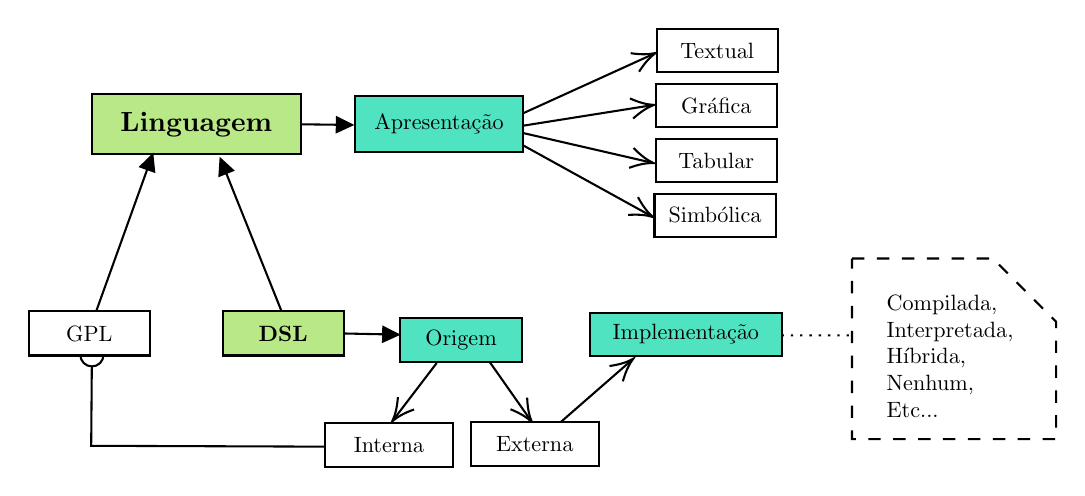
\begin{tikzpicture}[x=0.75pt,y=0.75pt,yscale=-1,xscale=1]
%uncomment if require: \path (0,408); %set diagram left start at 0, and has height of 408

%Shape: Rectangle [id:dp5982497232353539] 
\draw  [fill={rgb, 255:red, 184; green, 233; blue, 134 }  ,fill opacity=1 ] (43.96,49.84) -- (144.49,49.84) -- (144.49,78.83) -- (43.96,78.83) -- cycle ;
%Shape: Rectangle [id:dp8004700532925917] 
\draw  [fill={rgb, 255:red, 255; green, 255; blue, 255 }  ,fill opacity=1 ] (13.5,154.48) -- (71.89,154.48) -- (71.89,175.74) -- (13.5,175.74) -- cycle ;
%Shape: Rectangle [id:dp6645135942832383] 
\draw  [fill={rgb, 255:red, 184; green, 233; blue, 134 }  ,fill opacity=1 ] (106.92,154.48) -- (165.31,154.48) -- (165.31,175.74) -- (106.92,175.74) -- cycle ;
%Straight Lines [id:da940322594025554] 
\draw [fill={rgb, 255:red, 255; green, 255; blue, 255 }  ,fill opacity=1 ]   (45.99,154.48) -- (72.82,79.88) ;
\draw [shift={(73.5,78)}, rotate = 469.78] [fill={rgb, 255:red, 0; green, 0; blue, 0 }  ][line width=0.75]  [draw opacity=0] (8.93,-4.29) -- (0,0) -- (8.93,4.29) -- cycle    ;

%Straight Lines [id:da03980255509652442] 
\draw [fill={rgb, 255:red, 255; green, 255; blue, 255 }  ,fill opacity=1 ]   (135.35,154.48) -- (106.24,81.86) ;
\draw [shift={(105.5,80)}, rotate = 428.15999999999997] [fill={rgb, 255:red, 0; green, 0; blue, 0 }  ][line width=0.75]  [draw opacity=0] (8.93,-4.29) -- (0,0) -- (8.93,4.29) -- cycle    ;

%Shape: Rectangle [id:dp10111042590582864] 
\draw  [fill={rgb, 255:red, 80; green, 227; blue, 194 }  ,fill opacity=1 ] (192.6,157.7) -- (250.99,157.7) -- (250.99,178.64) -- (192.6,178.64) -- cycle ;
%Straight Lines [id:da05450643799113308] 
\draw [line width=0.75]    (165,165.11) -- (190.7,165.65) ;
\draw [shift={(192.7,165.69)}, rotate = 181.2] [fill={rgb, 255:red, 0; green, 0; blue, 0 }  ][line width=0.75]  [draw opacity=0] (8.93,-4.29) -- (0,0) -- (8.93,4.29) -- cycle    ;

%Shape: Rectangle [id:dp7588912578537257] 
\draw  [fill={rgb, 255:red, 80; green, 227; blue, 194 }  ,fill opacity=1 ] (170.72,50.8) -- (251.62,50.8) -- (251.62,77.86) -- (170.72,77.86) -- cycle ;
%Straight Lines [id:da14516072645219635] 
\draw    (168.39,64.63) -- (144.49,64.33) ;

\draw [shift={(170.38,64.65)}, rotate = 180.71] [fill={rgb, 255:red, 0; green, 0; blue, 0 }  ][line width=0.75]  [draw opacity=0] (8.93,-4.29) -- (0,0) -- (8.93,4.29) -- cycle    ;
%Straight Lines [id:da9230572726153299] 
\draw    (189.85,205.85) -- (210.08,179.33) ;

\draw [shift={(188.64,207.44)}, rotate = 307.34] [color={rgb, 255:red, 0; green, 0; blue, 0 }  ][line width=0.75]    (10.93,-4.9) .. controls (6.95,-2.3) and (3.31,-0.67) .. (0,0) .. controls (3.31,0.67) and (6.95,2.3) .. (10.93,4.9)   ;
%Straight Lines [id:da8579766023100592] 
\draw    (254.77,206.13) -- (235.75,179.06) ;

\draw [shift={(255.92,207.77)}, rotate = 234.92] [color={rgb, 255:red, 0; green, 0; blue, 0 }  ][line width=0.75]    (10.93,-4.9) .. controls (6.95,-2.3) and (3.31,-0.67) .. (0,0) .. controls (3.31,0.67) and (6.95,2.3) .. (10.93,4.9)   ;
%Straight Lines [id:da5652440770199652] 
\draw    (313.68,30.83) -- (251.75,59) ;

\draw [shift={(315.5,30)}, rotate = 155.54] [color={rgb, 255:red, 0; green, 0; blue, 0 }  ][line width=0.75]    (10.93,-4.9) .. controls (6.95,-2.3) and (3.31,-0.67) .. (0,0) .. controls (3.31,0.67) and (6.95,2.3) .. (10.93,4.9)   ;
%Straight Lines [id:da8514029171064224] 
\draw    (312.77,55.31) -- (251.75,65) ;

\draw [shift={(314.75,55)}, rotate = 170.98] [color={rgb, 255:red, 0; green, 0; blue, 0 }  ][line width=0.75]    (10.93,-4.9) .. controls (6.95,-2.3) and (3.31,-0.67) .. (0,0) .. controls (3.31,0.67) and (6.95,2.3) .. (10.93,4.9)   ;
%Shape: Rectangle [id:dp17415476114279294] 
\draw  [fill={rgb, 255:red, 255; green, 255; blue, 255 }  ,fill opacity=1 ] (226.45,207.96) -- (288.15,207.96) -- (288.15,228.89) -- (226.45,228.89) -- cycle ;
%Shape: Rectangle [id:dp5862398976742373] 
\draw  [fill={rgb, 255:red, 255; green, 255; blue, 255 }  ,fill opacity=1 ] (156.18,208.34) -- (217.88,208.34) -- (217.88,229.28) -- (156.18,229.28) -- cycle ;
%Shape: Rectangle [id:dp9794697115134454] 
\draw  [fill={rgb, 255:red, 255; green, 255; blue, 255 }  ,fill opacity=1 ] (315.61,44.77) -- (373.99,44.77) -- (373.99,65.71) -- (315.61,65.71) -- cycle ;
%Shape: Rectangle [id:dp07595309219569546] 
\draw  [fill={rgb, 255:red, 255; green, 255; blue, 255 }  ,fill opacity=1 ] (316.01,18.28) -- (374.4,18.28) -- (374.4,39.21) -- (316.01,39.21) -- cycle ;
%Shape: Rectangle [id:dp9653431753711184] 
\draw  [fill={rgb, 255:red, 80; green, 227; blue, 194 }  ,fill opacity=1 ] (283.98,155.09) -- (376.25,155.09) -- (376.25,176.03) -- (283.98,176.03) -- cycle ;
%Straight Lines [id:da6861278088536416] 
\draw    (269.62,207.98) -- (303.26,178.62) ;
\draw [shift={(304.76,177.3)}, rotate = 498.88] [color={rgb, 255:red, 0; green, 0; blue, 0 }  ][line width=0.75]    (10.93,-4.9) .. controls (6.95,-2.3) and (3.31,-0.67) .. (0,0) .. controls (3.31,0.67) and (6.95,2.3) .. (10.93,4.9)   ;

%Snip Single Corner Rect [id:dp83600176031787] 
\draw  [fill={rgb, 255:red, 255; green, 255; blue, 255 }  ,fill opacity=1 ][dash pattern={on 4.5pt off 4.5pt}] (410.17,129) -- (478.05,129) -- (508.5,159.45) -- (508.5,216) -- (410.17,216) -- cycle ;
%Straight Lines [id:da3854711457144977] 
\draw    (43.9,180.98) -- (43.6,219.23) -- (156.11,219.64) ;

\draw [shift={(43.9,180.98)}, rotate = 270.45] [color={rgb, 255:red, 0; green, 0; blue, 0 }  ][line width=0.75]      (5.59,-5.59) .. controls (2.5,-5.59) and (0,-3.09) .. (0,0) .. controls (0,3.09) and (2.5,5.59) .. (5.59,5.59) ;
%Straight Lines [id:da5105912486039843] 
\draw  [dash pattern={on 0.84pt off 2.51pt}]  (376.25,166.05) -- (409.5,166) ;


%Shape: Rectangle [id:dp1357804439753172] 
\draw  [fill={rgb, 255:red, 255; green, 255; blue, 255 }  ,fill opacity=1 ] (315.01,97.71) -- (373.4,97.71) -- (373.4,118.65) -- (315.01,118.65) -- cycle ;
%Shape: Rectangle [id:dp15166217408811944] 
\draw  [fill={rgb, 255:red, 255; green, 255; blue, 255 }  ,fill opacity=1 ] (315.51,71.28) -- (373.9,71.28) -- (373.9,92.21) -- (315.51,92.21) -- cycle ;
%Straight Lines [id:da2984867724600362] 
\draw    (312.55,82.55) -- (251.62,68.52) ;

\draw [shift={(314.5,83)}, rotate = 192.97] [color={rgb, 255:red, 0; green, 0; blue, 0 }  ][line width=0.75]    (10.93,-4.9) .. controls (6.95,-2.3) and (3.31,-0.67) .. (0,0) .. controls (3.31,0.67) and (6.95,2.3) .. (10.93,4.9)   ;
%Straight Lines [id:da44578022002737083] 
\draw    (312.5,108.03) -- (251.75,74.5) ;

\draw [shift={(314.25,109)}, rotate = 208.9] [color={rgb, 255:red, 0; green, 0; blue, 0 }  ][line width=0.75]    (10.93,-4.9) .. controls (6.95,-2.3) and (3.31,-0.67) .. (0,0) .. controls (3.31,0.67) and (6.95,2.3) .. (10.93,4.9)   ;

% Text Node
\draw (94.23,64.33) node [scale=1] [align=left] {\textbf{Linguagem}};
% Text Node
\draw (42.69,165.11) node [scale=0.8] [align=left] {GPL};
% Text Node
\draw (136.11,165.11) node [scale=0.8] [align=left] {\textbf{DSL}};
% Text Node
\draw (221.79,168.17) node [scale=0.8] [align=left] {Origem};
% Text Node
\draw (257.3,218.42) node [scale=0.8] [align=left] {Externa};
% Text Node
\draw (187.03,218.81) node [scale=0.8] [align=left] {Interna};
% Text Node
\draw (344.8,55.24) node [scale=0.8] [align=left] {Gráfica};
% Text Node
\draw (345.21,28.75) node [scale=0.8] [align=left] {Textual};
% Text Node
\draw (211.17,64.33) node [scale=0.8] [align=left] {Apresentação};
% Text Node
\draw (330.11,165.56) node [scale=0.8] [align=left] {Implementação};
% Text Node
\draw (457.39,176.08) node [scale=0.8] [align=left] {Compilada, \\Interpretada,\\Híbrida, \\Nenhum, \\Etc...};
% Text Node
\draw (344.21,108.18) node [scale=0.8] [align=left] {Simbólica};
% Text Node
\draw (344.71,81.75) node [scale=0.8] [align=left] {Tabular};


\end{tikzpicture}

    \label{fig:ClassDSL}
    \fonte{Adaptado de  \citeonline{Faveri:2013}.}
\end{figure}
    
Uma \ac{DSL} \textbf{interna} é projetada a partir das regras sintáticas e semânticas da gramática de uma linguagem já existente, podendo ser essa uma linguagem de propósito geral, do inglês \ac{GPL}, ou outra \ac{DSL}. 
Sendo assim, para seu funcionamento correto uma \ac{DSL} interna acaba transferindo todas as atividades de verificação léxica, sintática, semântica e de transformação de código ao compilador da linguagem hospedeira.

Uma \ac{DSL} \textbf{externa} é uma linguagem com sintaxe distinta e que depende de uma infraestrutura própria para a análise léxica, sintática, semântica, interpretação, compilação, otimização e geração de código. 
Se comparada a uma \ac{GPL}, uma \ac{DSL} externa possui especificidades similares, porém seus recursos são restritos ao domínio de aplicação para o qual a linguagem é projetada.
    
No que diz respeito a dimensão de \textbf{aparência}, uma \ac{DSL} pode ser classificada como \textbf{textual}, \textbf{gráfica}, \textbf{tabular} e \textbf{simbólica}. 
Quando no formato textual as \acp{DSL} permitem que o domínio seja expressado com caracteres, os quais são então combinados gerando palavras, expressões, sentenças e instruções que seguem as regras gramaticais previamente estabelecidas na linguagem. 
As \acp{DSL} não textuais seguem a mesma lógica, mas utilizando-se de modelos gráficos para permitir que o usuário possa expressar conhecimento de domínio com um maior nível de compreensão e empregando para tal o uso de símbolos, tabelas, figuras e conectores. 
    
E finalmente, no que se refere a dimensão de \textbf{implementação}, as \acp{DSL} podem ser classificadas tendo em vista a perspectiva de sua execução. 
Essas classificações formam quatro grupos: 
(i) \acp{DSL} de execução bem definidas (\textit{e.g.} Excel Macro Language); 
(ii) \acp{DSL} que servem de entrada para geradores de aplicação; 
(iii) \acp{DSL} não executáveis mas úteis como entrada de geradores de aplicação; 
(iv) \acp{DSL} não projetadas para serem executadas.

Em geral o principal aspecto levado em consideração para a construção de uma \acp{DSL} deve ser a sua \textbf{origem} pois cada abordagem apresenta vantagens e desvantagens específicas que são inerentes a cada tipo \cite{Fowler:2010}. 
Apesar das \acp{DSL} externas poderem ter um esforço associado a sua construção muitas vezes maior do que o de uma \ac{DSL} interna, atualmente existem ferramentas que dão grande suporte a construção de \acp{DSL}. 
Estas ferramentas são conhecidas como \acp{LW} e aplicam conceitos de programação orientada a linguagens, fornecendo um nível de abstração maior no que diz respeito as questões complexas de infraestrutura \cite{Fowler:2005}.
    
    
%#################################################################    
\subsection{\textit{Language Workbenches}} \label{ssec:LW}
%#################################################################

O desenvolvimento de uma \ac{DSL} não é tarefa trivial, pois como são linguagens de programação possuem uma sintaxe que é, por consequência lógica, definida por uma gramática. 
Desta forma, se faz necessária a utilização de ferramentas que suportem a definição dos conceitos para a nova linguagem \cite{Fowler:2005}.

Os \acp{LW} são ferramentas que fornecem mecanismos de infraestrutura para a implementação de linguagens de programação, tornando assim a criação de linguagens mais acessível \cite{Wachsmuth:2014}. 
Entre os mecanismos fornecidos nesses ambientes está a formatação automática, validação com base nas restrições descritas na gramática, \textit{syntax highlighting}\footnote{Realce de código-fonte com cor, negrito, etc. Serve para indicar sua estrutura sintática.} e \textit{syntax completion}\footnote{Uma função, como em um mecanismo de busca, que fornece uma ou mais opções de palavras reservadas previstas na gramática a partir dos caracteres que um usuário já inseriu.}. 
A seguir são citados três dos mais conhecidos \acp{LW} da atualidade:

\begin{itemize}
    \item \textbf{Xtext:} lançado em 2006, o Xtext é um \textit{framework} de código aberto para o desenvolvimento linguagens de programação textuais, com integração com o ambiente de desenvolvimento integrado, do inglês \ac{IDE}, Eclipse. 
    Para especificar uma linguagem, o desenvolvedor descreve uma gramática no Xtext. 
    Essa gramática descreve como um modelo \textit{Ecore} deve ser derivado de uma notação textual. 
    A partir dessa definição, um gerador de código deriva um analisador ANTLR e as classes para o modelo de objetos. 
    O Xtext também tem um gerador Xtend editável, o que dá a capacidade de se gerar código para qualquer outra gramática. 
    O Xtext inclui recursos inerentes ao \ac{IDE} Eclipse como \textit{syntax highlighting}, \textit{code completion}, \textit{static analysis}, \textit{source-code navigation} e outros. 
    Atualmente está na versão 2.17.1.
    
    \item \textbf{JetBrains MPS:} o JetBrains MPS é um sistema desenvolvido pela JetBrains, empresa da República Tcheca, que usa edição projetiva. 
    Essa abordagem permite aos desenvolvedores uma melhor compreensão, o que a diferencia de outros \acp{LW}. 
    Também possui funções comuns de \acp{IDE} integrado a seu ambiente de desenvolvimento. 
    Está atualmente na versão 2019.1.1 sob a licença Apache 2.0.
    
    \item \textbf{MetaEdit+:} o MetaEdit+ é \ac{LW} proprietário desenvolvido pela companhia finlandesa MetaCase para criar e utilizar \acp{DSL}. 
    Possui duas versões nomeadamente \textit{MetaEdit+ Workbench} e \textit{MetaEdit Modeler}. 
    O \textit{Workbench} inclui ferramentas para projetar e usar/testar linguagens de modelagem enquanto o Modeler inclui ferramentas para se utilizar linguagens de modelagem. 
    Normalmente, o \textit{MetaEdit+ Workbench} é usado pelos desenvolvedores que projetam uma \ac{DSL} do domínio para um projeto. 
    Em seguida, essa linguagem de modelagem é usada para desenvolver produtos finais com o apoio do \textit{MetaEdit+ Modeler}. 
    Atualmente está na versão 5.5 SR1.
\end{itemize}


%#################################################################
\section{Trabalhos Relacionados} \label{sec:TrabRelacionados}
%#################################################################

Essa seção descreve os trabalhos de maior representatividade para o objeto deste estudo. 
Uma vez que a proposta envolve a construção de uma ferramenta que implemente uma \ac{DSL} textual, e após a pesquisa descrita no \autoref{mapeamentoLiteratura} deste estudo, selecionou-se propostas e ferramentas que mais se aproximam do objetivo final deste trabalho.

O trabalho de \citeonline{Dimitrieski:2015}, desenvolvido na universidade de Novi Sad na Sérvia, apresenta uma ferramenta chamada \textit{System Modeling Tool} (MIST). 
Essa ferramenta utiliza uma \ac{DSL} chamada EERDSL, uma linguagem com base no modelo aprimorado de entidade-relacionamento, do inglês \ac{EER}.
A MIST apresenta uma abordagem de modelagem bidirecional (gráfica e textual) de modelagem de \acp{BD}. 
O autor discute que tal decisão tem como motivo o entendimento de que preferência sobre a abordagem de modelagem utilizada pode depender do domínio do problema, do conhecimento e das preferências pessoais de um projetista de \ac{BD}. 
Apresenta também uma experiência anterior, onde foi construído uma ferramenta de modelagem com uma abordagem baseada em formulários. 
A partir dos resultados obtidos nesta experiência, foi concebida a ideia da MIST. 
O propósito da ferramenta é a aplicação tanto no mercado profissional quanto para o ensino de projeto e modelagem de \ac{BD} no meio acadêmico. 
A MIST foi desenvolvida com o auxílio do Xtext para a notação da \ac{DSL} textual, e inicialmente a Eugene e posteriormente a Sirius para a sua versão gráfica. 
A MIST ainda oferece suporte à geração de código \ac{SQL}.

O \textit{dbdiagram.io}\footnote{https://dbdiagram.io/} é uma ferramenta \textit{Web} gratuita para o desenho de \acp{DER}, desenvolvida por uma empresa de Singapura, com uma abordagem textual que implementa uma \ac{DSL} própria.
Esta \ac{DSL} utiliza um modelo muito próximo do lógico. 
O diferencial da ferramenta é sua rápida curva de aprendizagem e, além disso, a apresentação de uma representação gráfica do que está sendo modelado.
A apresentação dos elementos do diagrama pode ser organizada livremente pelo usuário em tempo real. 
Entretanto é importante se salientar que toda a modelagem de fato é feita de modo textual. 
A ferramenta ainda oferece a geração automática de código \ac{SQL}.

Da mesma forma, a \textit{QuickDBD}\footnote{https://quickdatabasediagrams.com/}, desenvolvida por uma empresa na Irlanda, é uma ferrramenta \textit{Web} com exatamente o mesmo modo operacional que a \textit{dbdiagram.io}, também implementando uma \ac{DSL} textual própria para modelagem de \acp{BD}.
Contudo é uma ferramenta proprietária, ou seja, paga e com o foco declaradamente na indústria. 
Ambas as ferramentas são muito similares também quanto a geração de representações gráficas da modelagem e apresentam diversos argumentos para sua adoção, como a rápida compreensão de suas \acp{DSL}, a perspectiva de realização de trabalhos fluídos, o acesso de qualquer plataforma e o compartilhamento dos modelos com outros usuários.

Finalmente, pode-se citar a ferramenta \textit{Web} gratuita \textit{RelaX (Relational Algebra Calculator)}\footnote{https://dbis-uibk.github.io/relax/}. 
Esta ferramenta não foi encontrada no mapeamento, mas indicada por um pesquisador da área de \acp{DSL} e \acp{BD}. 
Trata-se de uma ferramenta desenvolvida na universidade de Innsbruck, na Áustria, e voltada ao ensino de álgebra relacional fazendo operações sobre bases de dados relacionais. 
Tem uma abordagem textual, utilizando uma \ac{DSL} chamada RelAlg, e apresentando inclusive duas perspectivas de operação: instruções de RelAlg e instruções em \ac{SQL}. 
A RelaX utiliza uma abordagem de modelo já em nível físico para operações, como as \acp{DDL} de construção e \acp{DML} para as consultas. 
Apesar de suas funcionalidades, a RelaX não se propõe a ser uma ferramenta de projeto e modelagem de \ac{BD}, mas de uso restrito ao ensino dentro da academia.

%#################################################################
\section{Lições do Capítulo} \label{sec:LicoesFundamentacaoTeorica}
%#################################################################

Os conceitos mais importantes para este trabalho foram apresentados neste capítulo. 
No geral foi necessário investigar dois grandes domínios, sendo eles: (i) projeto e modelagem de \ac{BD} e (ii) \ac{MDE}. 
Dentre os temas abordados destaca-se a Seção \ref{ssec:DSL}, a qual apresenta definições importantes para a compreensão do que é de fato uma \ac{DSL}. 
A Seção \ref{ssec:LW} também merece destaque pois cita alguns \acp{LW}, dentre eles o Xtext que acabou por ser a ferramenta selecionada para a construção do protótipo da proposta deste estudo.